\chapter{Fundamentos de semiconductores}

\section{La tabla periódica}

La tabla periódica de los elementos está ordenada en grupos y periodos, como se observa en la Figura \ref{tabla_periodica_acs}. Los \textbf{grupos} son las columnas, que describen elementos con estructuras electrónicas similares, generalmente con la misma cantidad de \textbf{electrones de valencia}. Por ejemplo, tanto el carbono, el silicio y el germanio son elementos del grupo 14 (también llamado grupo IV por convención) y tienen todos 4 electrones de valencia. Los \textbf{periodos} son las filas, y describen elementos con la misma cantidad de capas electrónicas. Todos los elementos de un periodo comparten el mismo número cuántico principal n.

\begin{figure}[H]
    \centering
    \begin{tabular}{|c|c|c|c|c|c|c|c|c|}
        \hline   & I  & II & III & IV & V & VI & VII & VIII \\
        \hline 1 & H  &    &    &    &    &    &    & He \\
        \hline 2 & Li & Be & B  & C  & N  & O  & F  & Ne \\
        \hline 3 & Na & Mg & Al & Si & P  & S  & Cl & Ar \\
        \hline 4 & K  & Ca & Ga & Ge & As & Se & Br & Kr \\
        \hline 5 & Rb & Sr & In & Sn & Sb & Te & I  & Xe \\
        \hline 6 & Cs & Ba & Tl & Pb & Bi & Po & At & Rn \\
        \hline 7 & Fr & Ra & Nh & Fl & Mc & Lv & Ts & Og \\
        \hline 
    \end{tabular}
    \caption{Tabla periódica de los elementos.}
    \label{tabla_periodica_acs}
\end{figure}



Un material puede ser \textbf{elemental} si tiene un único tipo de elemento, o \textbf{compuesto} si tiene al menos dos elementos distintos, en proporciones determinadas. Los materiales se pueden clasificar según sus propiedades físicas o químicas.

\section{Resistividad y conductividad}

Los materiales se clasifican según su \textbf{conductividad eléctrica ($\sigma$)}, que mide la capacidad para conducir electricidad, como metales, no metales o semiconductores. El silicio es el semiconductor más utilizado para fabricar transistores y circuitos integrados. En los semiconductores, la conductividad es intermedia y se puede ajustar con muy alta exactitud y precisión.

La resistencia eléctrica de un material se calcula como:

\[ R = \dfrac{\rho l}{A} = \dfrac{l}{\sigma A} \]

Donde $\rho$ es la resistividad del material, medida en $\Omega{}\cdot{}cm$, y $\sigma=1/\rho$ es la conductividad, medida en $S/cm$. La resistencia eléctrica depende de la geometría, mientras que la resistividad y la conductividad son constantes del material, sin importar la forma que tenga. 

En la Tabla \ref{tabla_resistividad_conductividad} se muestran los valores de resistividad y conductividad para algunos materiales comúnmente utilizados en la industria microelectrónica.

\begin{table}[H]
    \centering
    \caption{Resistividad y conductividad para algunos materiales utilizados en la industria microelectrónica, a una temperatura de 20 $^\circ{}C$ \cite{serway1998}.}
    \label{tabla_resistividad_conductividad}
    \begin{tabular}{|c|c|c|}
    \hline
        \textbf{Material} & \textbf{Resistividad ($\Omega{}\cdot{}cm$)} & \textbf{Conductividad ($S/cm$)} \\
        \hline 
        Oro (Au)        & $2.44\times{}10^{-6}$  & $4.10\times{}10^5$ \\
        Aluminio (Al)   & $2.82\times{}10^{-6}$  & $3.55\times{}10^5$ \\
        Cobre (Cu)	    & $1.70\times{}10^{-6}$  & $5.88\times{}10^5$ \\
        Silicio (Si)    & $6.40\times{}10^{3}$	 & $1.56\times{}10^{-4}$ \\
        Germanio (Ge)	& $4.60\times{}10^{2}$	 & $2.17\times{}10^{-2}$ \\
        Vidrio (SiO\textsubscript{2}) & $10^{12}$ - $10^{16}$ & $10^{-12}$ - $10^{-16}$ \\
        \hline
    \end{tabular}
\end{table}

\section{Estructura atómica}

Los átomos en materiales sólidos forman enlaces con distintas configuraciones geométricas en el espacio. Existen sólidos \textbf{cristalinos}, donde los átomos mantienen una estructura ordenada regular en todo el volumen del cristal, y es la misma en cualquier punto. Los sólidos \textbf{amorfos} son aquellos donde sus átomos no forman ningún patrón ordenado. Los sólidos \textbf{policristalinos} tienen secciones cristalinas independientes entre sí. Estas tres configuraciones se muestran en la Figura 4.

\begin{figure}[H]
    \centering
    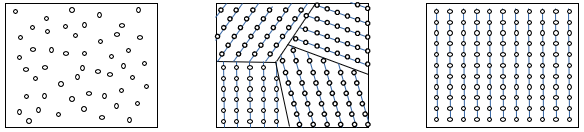
\includegraphics{figuras/cristalinidad.png}
    
    a) Amorfos \hspace{2.5cm} b) Policristalinos \hspace{2.5cm} c) Cristalinos
    
    \caption{Clasificación de materiales según su estructura atómica (grado de cristalinidad).}
    \label{cristalinidad}
\end{figure}

A nivel industrial se utilizan mayoritariamente el silicio (Si) y el germanio (Ge) para la construcción de dispositivos electrónicos, especialmente el silicio, que suele ser más abundante en la naturaleza. El silicio tiene cuatro electrones de valencia, dispuestos en una configuración cristalina similar a la del diamante y la zinc blenda. Esta configuración se representa por ocho átomos en las esquinas, seis átomos en las caras y cuatro átomos internos.

\section{El modelo atómico de Bohr}

Los modelos atómicos más conocidos son el modelo atómico de Dalton, Thomson, Rutherford, Bohr y Schrödinger. El modelo de Schrödinger describe la probabilidad de encontrar un electrón en el espacio. La solución de la ecuación de Schrödinger da como resultado niveles discretos de energía, y orbitales. 

En el año 1913 Niels Bohr y Ernest Rutherford plantean un enfoque para definir la estructura atómica de los elementos, donde se ubica a los electrones distribuidos en orbitas estables y bien definidas alrededor del átomo; cada electrón solamente puede tener ciertos valores de momento angular. En el modelo atómico de Bohr, los electrones se distribuyen en órbitas definidas alrededor del núcleo, como se observa en la Figura \ref{modelo_bohr} para el átomo de hidrógeno y el átomo de silicio. 

\begin{figure}[H]
    \centering
    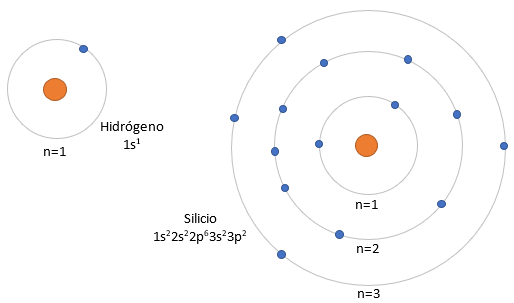
\includegraphics{figuras/modelo_bohr.png}
    \caption{Modelos atómicos para el átomo de hidrógeno y el átomo de silicio.}
    \label{modelo_bohr}
\end{figure}


\section{Modelo de enlaces}

El silicio tiene cuatro electrones de valencia, y forma cuatro enlaces covalentes con sus átomos más cercanos, para compartir electrones y llegar a cumplir con la \textbf{regla del octeto}: la configuración más estable de un átomo tiene ocho electrones en su último nivel de energía, similar a la configuración de un gas noble. En cada \textbf{enlace covalente} se comparten dos electrones, de manera que cada átomo de silicio cuenta con cuatro electrones propios y cuatro electrones compartidos por los átomos vecinos \cite{b1}. Esto se visualiza por medio del modelo de enlaces, que se muestra en la Figura \ref{fig:EstructuraCristalinaSi} para el silicio a una temperatura de 0 K. Cada átomo se representa por un círculo, y cada electrón compartido se representa por una línea. 

Es válido considerar la distancia entre átomos como una distancia equidistante entre todos ellos y definida por un enlace de dos electrones. Si se considera un cuarteto de átomos vecinos, se podría trazar un cuadrado desde el centro de cada uno de los átomos y ese cuadrado contendría exactamente un átomo compuesto por cuatro cuartos de átomo.


\begin{figure}[H]
  \centering
  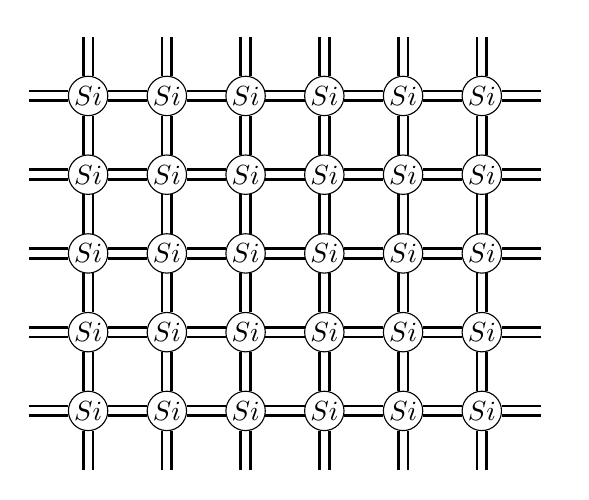
\begin{tikzpicture}[xscale=0.25, yscale=0.25]
    %------------Horizontales----------
    \foreach \x in {-11,-7,...,13} {
        \foreach \y in {-8,-4,...,8} {
            \draw[line width=1pt](\x,\y-0.25)--(2+\x,\y-0.25)node[right] {};
            \draw[line width=1pt](\x,\y+0.25)--(2+\x,\y+0.25)node[right] {};
        }
    }
    %-------------Verticales-----------
    \foreach \y in {-11,-7,...,9} {
        \foreach \x in {-8,-4,...,12} {
            \draw[line width=1pt](\x-0.25,\y)--(\x-0.25,\y+2)node[right] {};
            \draw[line width=1pt](\x+0.25,\y)--(\x+0.25,\y+2)node[right] {};
        }
    }
    %------------Circulos--------------
    \foreach \x in {-8,-4,...,12} {
            \foreach \y in {-8,-4,...,8} {
                \draw (\x,\y) circle(1) node {$Si$};
        }
    }
    %\draw [ultra thick, red   ] (0, 0.0) -- (2, 0.0);
    %\node[fill=blue] at (0.5,1) {text};
  \end{tikzpicture}
  \caption{Estructura cristalina del silicio en dos dimensiones, a un temperatura de 0 K.}
  \label{fig:EstructuraCristalinaSi}
\end{figure}

A una temperatura de cero absoluto (T = 0 K), todos los electrones del silicio están formando enlaces covalentes, no hay electrones libres y la conductividad del silicio es nula. El silicio es un aislante a 0 K. 


\section{Generación y recombinación}

Conforme aumenta la temperatura, algunos enlaces se rompen por \textbf{generación} térmica. En este proceso se crea un electrón libre, que es un \textbf{portador de carga} negativa, y se produce un espacio libre en la estructura cristalina. Este espacio se conoce como \textbf{hueco}. La carga eléctrica de un electrón es $q_e=-1.602\times{}10^{-19}\ C$.

Un hueco es un espacio vacío que ha dejado un electrón al romperse un enlace, es decir, los enlaces se encuentran en enlaces incompletos y se genera un par electrón-hueco. Un hueco es capaz de absorber a un electrón, lo cual describe la recombinación de un par electrón-hueco.

El proceso de generación térmica se ilustra en la Figura \ref{generacion_recombinacion_1}:

\begin{figure}[H]
    \centering
    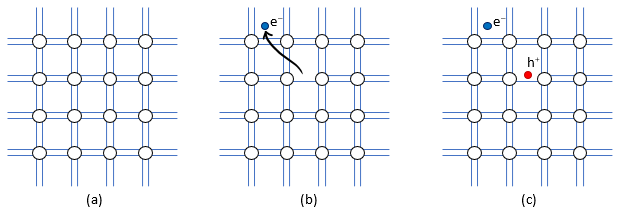
\includegraphics{figuras/generacion_y_recombinacion_1.png}
    \caption{Modelo de enlaces para silicio: (a) para una temperatura T = 0 K, todos los enlaces están completos. (b) al aumentar la temperatura se rompe un enlace, (c) representación de un hueco.}
    \label{generacion_recombinacion_1}
\end{figure}

Cualquier electrón libre puede llegar a ocupar el espacio vacío, y reconstruir el enlace faltante. Esto aniquila tanto al electrón como al hueco, en el proceso llamado \textbf{recombinación}. Debido a que el proceso de recombinación elimina la carga eléctrica libre, al hueco se le asigna una carga eléctrica neta equivalente positiva, que es $q_h=+1.602\times{}10^{-19}\ C$.

Tanto el electrón como el hueco se pueden representar como partículas móviles con carga. El flujo de electrones produce una corriente eléctrica. Sin embargo, en semiconductores es importante destacar que el flujo de huecos también produce una corriente eléctrica. En la Figura \ref{generacion_recombinacion_2} se observa el flujo de electrones y de huecos.

\begin{figure}[H]
    \centering
    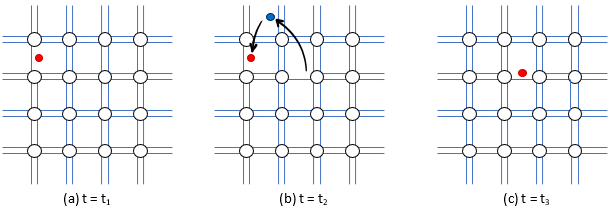
\includegraphics{figuras/generacion_y_recombinacion_2.png}
    \caption{Movimiento de electrones y de huecos para ilustrar ambas corrientes. En esta secuencia, un enlace se rompe, se libera un electrón, este electrón ocupa la posición del hueco original, y queda un hueco en otra posición. El electrón se mueve hacia la izquierda, el hueco se mueve hacia la derecha.}
    \label{generacion_recombinacion_2}
\end{figure}

El proceso de generación y recombinación ocurre constantemente en todas las posiciones del cristal, con velocidades distintas, de manera que a temperatura ambiente existe una cantidad finita de electrones y huecos libres. Estos son los \textbf{portadores de carga} disponibles para la conducción, que definen la conductividad y la resistividad del material.

Si la temperatura aumenta, se rompen más enlaces que los que se recombinan, creando más pares electrón-hueco por generación térmica y aumentando la conductividad del material. Por el contrario, si la temperatura disminuye, los electrones y huecos se recombinan más frecuentemente que el proceso de generación, disminuyendo la conductividad del material.

La conductividad de un semiconductor depende de la temperatura, porque existe una cierta cantidad de electrones y huecos disponibles para la conducción, que es función de la temperatura. La cantidad de portadores libres por centímetro cúbico de material se denomina \textbf{concentración de portadores libres}.


\newpage
\section{El voltaje térmico}

Para romper un enlace covalente se necesita energía. La cantidad de energía que se requiere para romper un enlace covalente depende del material, y se denomina \textbf{energía de la banda prohibida} $E_g$. Para el silicio esta constante tiene un valor de $E_g=1.12\ eV$ y para el germanio $E_g=0.66\ eV$.

La temperatura introduce energía en el material, y la cantidad de energía que se introduce es proporcional a la \textbf{constante de Boltzmann} $k=1.38\times{}10^{-23}\ J/K$. De esta manera, la energía térmica se calcula como $E_T=kT$. La tensión se define como $1\ V = 1\ J/1\ C$, de manera que es posible calcular el \textbf{voltaje térmico} $V_T$ como:

\[V_T=\dfrac{kT}{q}\]

A temperatura ambiente (T = 300 K), el voltaje térmico es de 25.85 mV.


\section{Masa efectiva de los portadores de carga}

Al aplicar un campo eléctrico, un electrón en el vacío experimenta una fuerza y una aceleración constante. La relación entre las variables se describe con las siguientes ecuaciones, donde la masa para un electrón es $m_0=9.1\times{}10^{-31}\ kg$:

\[ \vec{F} = q_e \times \vec{E} = m_0 \times \vec{a} = m_0 \times \dfrac{d\vec{v}}{dt} \]

En un material como el silicio, la fuerza que experimenta la partícula es la misma, pero la aceleración es distinta, debido a que existen obstáculos para el movimiento libre del electrón dentro de la estructura cristalina. El electrón encuentra otros átomos de la estructura cristalina en su camino, y puede experimentar fuerzas de atracción o repulsión con otros portadores de carga. Para modelar este efecto de la disminución de velocidad en un sólido y poder continuar modelando el movimiento del electrón por medio de la mecánica clásica, se define la \textbf{masa efectiva} del electrón, como un ajuste a la masa original que considera el movimiento del electrón dentro de un sólido. De este modo, se reescribe la ecuación anterior, donde $m_e^*$ es la masa efectiva del electrón, definida para un material específico.

Las mismas ecuaciones se pueden utilizar para describir el movimiento de huecos, aunque para este segundo caso es necesario definir una masa para un espacio vacío en la estructura cristalina. El hueco no debería tener masa, pero se le asigna una masa para poder describir su movimiento por medio de la mecánica clásica. La masa efectiva de los electrones y los huecos en distintos materiales se expresa como una fracción de la masa original, y se resume en la Tabla \ref{tabla_masas_efectivas}. 

\begin{table}[H]
    \centering
    \caption{Masas efectivas para el electrón y el hueco \cite{b7}.}
    \label{tabla_masas_efectivas}
    \begin{tabular}{|c|c|c|}
        \hline \textbf{Material} & \textbf{$m_e^*/m_0$} & \textbf{$m_h^*/m_0$} \\
        \hline Silicio (Si) & 1.18 & 0.81 \\
        Germanio (Ge) & 0.55 & 0.36 \\
        Arseniuro de galio (GaAs) & 0.066 & 0.52 \\
        \hline
    \end{tabular}
\end{table}


\section{Concentración intrínseca de portadores}

Un semiconductor \textbf{intrínseco} es aquel que tiene un alto nivel de pureza, es decir, un material en el cual casi la totalidad de átomos son del mismo tipo. En el caso del silicio, es posible obtener niveles de pureza del 99.9999999\% (pureza de ``nueve nueves'').

Para una muestra de silicio intrínseco a temperatura ambiente, existe una cierta cantidad de electrones y huecos libres disponibles para la conducción. La \textbf{concentración de electrones libres por centímetro cúbico} se define como $n$, y la \textbf{concentración de huecos libres por centímetro cúbico} se define como $p$. Debido a que en el silicio puro los portadores se crean en pares, la cantidad de electrones es igual a la de huecos ($n=p$), y el material tiene una carga eléctrica neta igual a cero. A esta propiedad se le conoce como \textbf{balance de cargas}.

La concentración intrínseca de electrones en función de la temperatura se calcula con la siguiente ecuación \cite{b11}:
%
\[ n_i = 2 \left( \dfrac{2 \pi m^*_e k T}{h^2} \right)^{3/2} \cdot e^{\dfrac{-E_g}{2kT}} \]
%
Donde $k$ es la constante de Boltzmann ($k=1.38\times{}10^{-23}\ J/K$), $h$ es la constante de Planck ($h=6.626\times{}10^{-34}\ J\cdot{}s$) y $E_g$ es la energía de la banda prohibida, que debe convertirse primero a Joules para que las unidades sean consistentes. Las unidades de $n_i$ son $m^{-3}$ y describe la cantidad de electrones libres por metro cúbico. 

\begin{figure}[H]
    \centering
    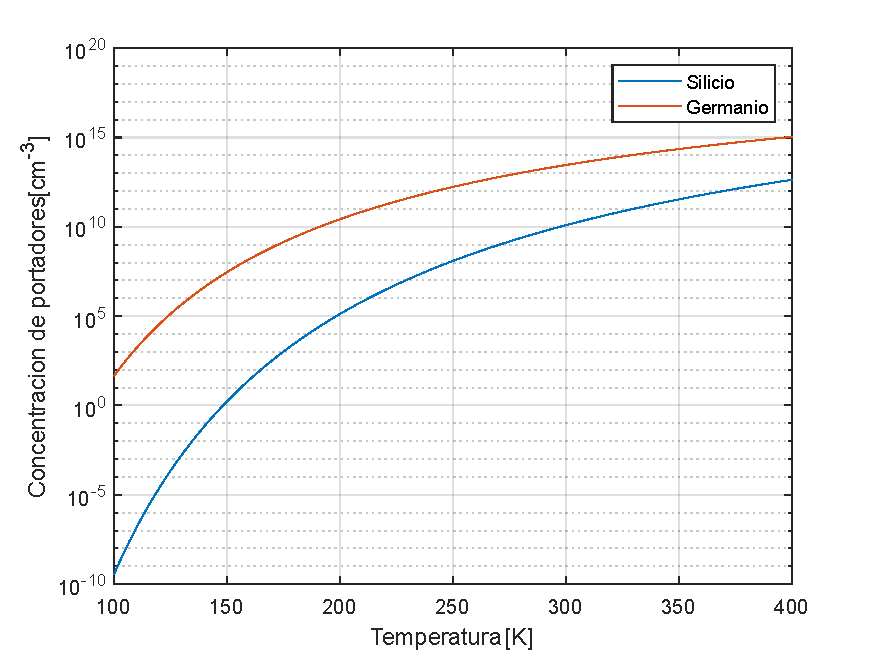
\includegraphics[width=14cm]{figuras/concentracion_intrinseca_portadores.pdf}
    \caption{Concentración intrínseca de portadores (electrones por centímetro cúbico) para el silicio y el germanio, en función de la temperatura en Kelvin.}
    \label{concentracion_intrinseca_vs_T}
\end{figure}

Generalmente las concentraciones se expresan en electrones por centímetro cúbico, por lo que es necesario multiplicar la ecuación anterior por un factor de $10^{-6}$ para obtener finalmente la concentración de electrones por centímetro cúbico. En la Figura \ref{concentracion_intrinseca_vs_T} se muestra la gráfica con las concentraciones de electrones para el silicio y el germanio, donde se observa que, para silicio, $n_i(300\ K) \approx 10^{10}\ cm^{-3}$.


\begin{ejemplo} % usar entorno para ejemplos...
Realice el análisis dimensional de la ecuación de $n_i(T)$, demuestre que el resultado está en $m^{-3}$ y demuestre que el factor de conversión requerido para convertir a $cm^{-3}$ es $10^{-6}$.
\end{ejemplo}

\begin{solucion} % ...y usar entorno para soluciones
Se sustituyen las unidades de cada variable:

\[ [n_i] = \left( \dfrac{[kg]\left[\dfrac{J}{K}\right][K]}{[Js]^2} \right)^{3/2} \cdot e^{\dfrac{[J]}{[J/K][K]}} \]

\[ [n_i] = \left(\dfrac{[kg][J]}{[J]^2 [s]^2} \right)^{3/2} \cdot{} e^1 \]

\[ [n_i] = \left( \dfrac{[kg]}{[J] [s]^2} \right)^{3/2} \cdot [1] \]

Donde $1\ J=1\ kg\cdot{}m^2/s^2$:

\[ [n_i] = \left( \dfrac{[kg]}{\left[ \dfrac{kg\cdot{}m^2}{s^2} \right] [s]^2} \right)^{3/2} \]

\[ [n_i] = \left( \dfrac{1}{[m^2]} \right)^{3/2} \]

\[ [n_i] = \dfrac{1}{[m^{6/2}]} \]

\[ [n_i] = \dfrac{1}{[m^3]} \]

Para pasar a centímetros cúbicos se aplica el factor de conversión:

\[ [n_i] = \dfrac{1}{[m^3]} \times \dfrac{[1\ m]^3}{[100\ cm]^3} \]

\[ [n_i] = \dfrac{1}{[m^3]} \times \dfrac{1\ [m^3]}{100^3\ [cm^3]} \]

\[ [n_i] = \dfrac{1}{10^6\ [cm^3]} \]

\[ [n_i] = 10^{-6}\ cm^{-3} \]
\end{solucion}

\newpage
\begin{ejemplo}
Determine la concentración intrínseca de electrones en el silicio a temperatura ambiente $T=300\ K$ y a una temperatura $T=310\ K$. Exprese el resultado en $cm^{-3}$.
\end{ejemplo}

\begin{solucion}
A temperatura ambiente $T=300\ K$:

\[ n_i = 2 \left( \dfrac{2 \pi (1.18\times{}9.1\times{}10^{-31}\ kg) (1.38\times{}10^{-23}\ J/K)(300\ K)}{(6.626\times{}10^{-34}\ Js)^2} \right)^{3/2} \cdot e^{\dfrac{-1.12\ eV}{2(8.617\times{}10^{-5}\ eV/K)(300\ K)}} \]

\[ n_i(300\ K) = 1.24\times{}10^{16}\ m^{-3} \]

\[ n_i(300\ K) = 1.24\times{}10^{10}\ cm^{-3} \]

A una temperatura $T=310\ K$:

\[ n_i = 2 \left( \dfrac{2 \pi (1.18\times{}9.1\times{}10^{-31}\ kg) (1.38\times{}10^{-23}\ J/K)(310\ K)}{(6.626\times{}10^{-34}\ Js)^2} \right)^{3/2} \cdot e^{\dfrac{-1.12\ eV}{2(8.617\times{}10^{-5}\ eV/K)(310\ K)}} \]

\[ n_i(300\ K) = 2.63\times{}10^{16}\ m^{-3} \]

\[ n_i(300\ K) = 2.63\times{}10^{10}\ cm^{-3} \]

Para un incremento de $10\ ^\circ{}C$, la concentración intrínseca de portadores se duplica.
\end{solucion}

\begin{ejemplo}
Calcule la temperatura a la cual la concentración intrínseca de portadores en el silicio es 10 veces la concentración intrínseca a temperatura ambiente. 
\end{ejemplo}

\begin{solucion}
Se quiere encontrar la temperatura $T_X$ tal que:

\[n_i(T_X) = 1.24\times{}10^{11}\ cm^{-3} = 1.24\times{}10^{17}\ m^{-3} \]

Por lo tanto, esta concentración se iguala a la ecuación:

\[ 1.24\times{}10^{17}\ m^{-3} = 2 \left( \dfrac{2 \pi m^*_e k T_X}{h^2} \right)^{3/2} \cdot e^{\dfrac{-E_g}{2kT_X}} \]

Donde se debe despejar $T_X$, lo cual no es tan sencillo. 

Se resuelve por aproximación numérica con la calculadora, presionando SHIFT+SOLVE:

\[ T_X=332.8\ K \]

\end{solucion}

\section{Concentración extrínseca de portadores}

La concentración de portadores en un material se puede modificar mediante \textbf{dopado}. Esta técnica consiste en adicionar átomos específicos de otros grupos de elementos a una red cristalina. 
Un material \textbf{extrínseco} es aquel al que se le han agregado impurezas específicas, con la finalidad de controlar la concentración de portadores. Los átomos dopantes más comunes son los elementos de los grupos 13 y 15 (elementos III-V), los cuales se muestran en la Tabla \ref{tabla_atomos_dopantes}. 

\begin{table}[H]
    \centering
    \caption{Dopantes comunes para silicio.}
    \label{tabla_atomos_dopantes}
    \begin{tabular}{|c|c|}
        \hline \textbf{Átomos aceptores} & \textbf{Átomos donadores} \\
        Dopado tipo p & Dopado tipo n \\
        \hline
        B  & N \\
        Al & P \\
        Ga & As \\
        In & Sb \\
        \hline
    \end{tabular}
\end{table}

Se llama \textbf{donador} a aquel átomo añadido que aporta electrones libres a la estructura cristalina, los donadores en general incrementan la concentración de electrones del material (\textbf{tipo n}). Por otro lado, se le conoce como \textbf{aceptor} a aquel átomo que incrementa la concentración de huecos al material (\textbf{tipo p}).

El efecto de agregar estos elementos se puede visualizar con el modelo de enlaces. En la Figura \ref{dopado_modelo_enlaces}(a) se muestra la estructura del silicio, donde se reemplazó un átomo de silicio por un \textbf{átomo donador} que tiene cinco electrones en la última órbita, de los cuales cuatro forman enlaces y el quinto electrón está débilmente ligado al núcleo. Este electrón extra se libera a temperatura ambiente, \textbf{ionizando} al átomo (convirtiéndolo en un átomo cargado eléctricamente positivo, al tener un electrón menos que la cantidad de protones en el núcleo), e incrementa la concentración de electrones libres, de modo que n aumenta. 

\begin{figure}[H]
    \centering
    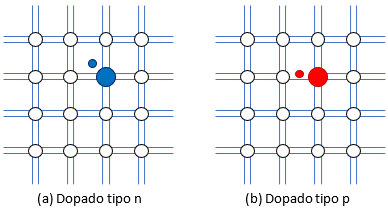
\includegraphics{figuras/modelo_enlaces_dopado.png}
    \caption{Modelo de enlaces para silicio con un único átomo dopante: (a) dopado con donadores y por lo tanto de tipo n, (b) dopado con aceptores y por lo tanto de tipo p.}
    \label{dopado_modelo_enlaces}
\end{figure}

\newpage
En la Figura \ref{dopado_modelo_enlaces}(b) se ilustra el proceso contrario: un \textbf{átomo aceptor} tiene sólo tres electrones en la última órbita, de modo que no puede formar los cuatro enlaces. Al formar solo tres enlaces, queda un espacio vacío en la estructura del cristal, que puede llegar a ser ocupado por otro electrón. Si se forma un enlace en esa posición, el átomo donador queda \textbf{ionizado} (convirtiéndolo en un átomo eléctricamente cargado con carga negativa, al tener un electrón más que la cantidad de protones en el núcleo). El electrón que ocupó el cuarto enlace proviene del cristal, y dejó un espacio vacío o hueco en alguna otra parte, por lo que el dopado con aceptores incrementa la concentración de huecos libres, aumentando p.

Las \textbf{energías de ionización} de los átomos dopantes son considerablemente pequeñas, y se sabe que, a temperatura ambiente, todos los átomos dopantes están ionizados completamente, por lo que los electrones o huecos que aportan pasan directamente a ser portadores libres.

\vspace{5mm}
\begin{tcolorbox}[sharp corners, colback=white, colframe=tec-blue, title=Ionización de átomos en cloruro de sodio]
\small El proceso de \textbf{ionización} generalmente ocurre a mayor escala entre átomos de metales y no metales, sin embargo también se produce entre semiconductores y materiales con números de valencia cercanos. Se produce cuando un átomo intercambia portadores con otro átomo o con el ambiente, adquiriendo así una carga, ya sea negativa o positiva.

Si se tuviese el caso donde un átomo de sodio, que tiene un electrón en su capa más externa, dona ese electrón a un átomo de cloro, que tiene 7 electrones en su capa más externa, entonces ambos átomos logran llenar sus capas externas. Después del intercambio, el átomo de sodio queda cargado de forma positiva y el átomo de Cloro queda cargado o ionizado de forma negativa, ambos se atraen ente sí.
\end{tcolorbox}


\section{Generación y recombinación}

Los mecanismos naturales para estabilizar un desbalance ocasionado por una perturbación al equilibrio de un semiconductor se conocen como \textbf{generación} (G) y \textbf{recombinación} (R). Las perturbaciones al estado de equilibrio (por ejemplo, una diferencia de potencial, un cambio de temperatura o la exposición a la luz) ocasionan ya sea un incremento o un decremento de la concentración de portadores respecto al valor de las concentraciones intrínsecas que el mismo semiconductor tiene en equilibrio.

La generación es el proceso en el que se crean electrones libres y huecos, mientras que la recombinación es el proceso inverso donde se eliminan electrones libres y huecos. Ambos mecanismos permiten la estabilización de las concentraciones para el caso en el que la perturbación se mantenga afectando al semiconductor. Además, se encargan de la remoción del exceso de concentración para el caso en el que la fuente de perturbación deja de afectar al semiconductor. Lo más común es que un semiconductor se vea permanentemente afectado por perturbaciones, por lo tanto dichos mecanismos forman parte de las características mostradas por un dispositivo semiconductor.

Para el caso donde un tipo de portador sea más abundante que el otro, se sabe que la tasa de recombinación es baja. Se puede intuir que, si la presencia de ambos tipos de portador es alta, se tiene una recombinación alta. Lo anterior nos lleva a definir a la recombinación como el producto entre los dos tipos de portador de un semiconductor y a una relación medible entre ellas (C) que será constante.   

\[ R = C \cdot n \cdot p \]

La generación se compone de dos tipos, la generación térmica ($G_{t}$) y la generación óptica ($G_{o}$). La primera se da cuando la temperatura es mayor al cero absoluto, es decir $T > 0\ K$, situación que aporta energía térmica y rompe enlaces covalentes, los electrones liberados dejan a su paso iones negativos, generando pares electrón-hueco. La generación por efecto óptico es producto de la iluminación que golpee al material, es independiente de la temperatura y debe provenir de una fuente apropiada; cuando los fotones generan energía suficiente para romper enlaces, generan a su vez pares de portadores.   

\[ G = G_{t} + G_{o} \]

Siguiendo con el ejemplo de perturbación por temperatura, el estado de equilibrio se alcanza cuando se llega a mantener la temperatura constante en algún punto y durante algún tiempo; es decir donde la tasa de $G$ y de $R$ es la misma, igualando así el numero de portadores negativos con el número de portadores positivos.

\[ n \cdot p =  \dfrac{G_{t} + G_{o}}{C} \]

En equilibrio no hay intercambio de energía con el medio, por lo que la concentración intrínseca de portadores se puede definir ya sea como la cantidad de portadores de carga negativos, o como la cantidad de portadores de carga positivos:

\[ n_{i} =  n = p \]

\section{Ley de acción de masas}

En la sección anterior se observó que, al dopar con átomos donadores, la concentración de electrones n aumenta. Sin embargo, la concentración de huecos p disminuye, porque los electrones, que ahora abundan en el cristal, empiezan a recombinarse con más frecuencia con los huecos.

En un semiconductor en \textbf{equilibrio térmico} (sin tensión aplicada, con temperatura constante y en ausencia de luz) y con dopado \textbf{no degenerado} (concentraciones de dopado menores a $10^{18}\ cm^{-3}$) se cumple \textbf{la ley de acción de masas}, que indica que la concentración intrínseca de portadores al cuadrado se mantiene constante:

\[ n_i^2 = n \cdot p \]

Si se agrega una \textbf{concentración de átomos dopantes donadores} $N_D$, medida en átomos/cm$^3$, y esta concentración es mucho más alta que la concentración intrínseca de electrones ($N_D \gg n_i$), entonces la cantidad de electrones libres se calcula como $n\approx{}N_D$. La cantidad de huecos libres se obtiene con la ley de acción de masas como $p=n_i^2/n$:

\[ n \approx N_D \]

\[ p \approx \dfrac{n_i^2}{N_D} \]

Si por el contrario se agrega una \textbf{concentración de átomos dopantes aceptores} $N_A$, medida en átomos/cm$^3$, y esta concentración de átomos dopantes es mucho mayor que la concentración intrínseca de electrones ($N_A \gg n_i$), entonces la cantidad de huecos libres se calcula como $p\approx{}N_A$. La cantidad de huecos libres se obtiene con la misma ley de acción de masas como $n=n_i^2/p$:

\[ p \approx N_A \]

\[ n \approx \dfrac{n_i^2}{N_A} \]

Para estos cálculos se ha asumido que el dopado es considerablemente fuerte, y que el material tiene un único tipo de dopado. Sin embargo, en ocasiones se requiere dopar con ambos tipos de átomos, en una técnica llamada compensación. Para ese caso se utiliza la ecuación de balance de cargas. 

\begin{ejemplo}
Una muestra de silicio se dopa con átomos de arsénico, con una concentración de dopado uniforme $N_D=10^{14}\ cm^{-3}$. ¿Qué tipo de dopado presenta la muestra? Determine las concentraciones de portadores $n$ y $p$.
\end{ejemplo}

\begin{solucion}
El arsénico es un átomo donador, que aumenta las concentraciones de electrones de la muestra. Por lo tanto, el material es de tipo n.

La concentración de electrones n es igual a la concentración de átomos dopantes:

\[ n \approx N_D \]

\[ n \approx 10^{14}\ cm^{-3} \]

La concentración de huecos p se calcula con la ley de acción de masas:

\[ p \approx \dfrac{n_i^2}{n} \]

\[ p \approx \dfrac{(10^{10})^2}{10^{14}} \]

\[ p \approx 10^6\ cm^{-3} \]
\end{solucion}


\newpage
\section{Neutralidad de carga}

En cualquier semiconductor en equilibrio térmico, la carga neta dentro del material es igual a cero, sin importar la cantidad de átomos dopantes. Esto sucede porque todos los átomos dopantes tienen la misma cantidad de electrones y protones, aunque aumenten la concentración de un tipo de portador y disminuyan la concentración del otro. La ecuación de \textbf{balance de cargas} (también conocida como neutralidad de carga) es la siguiente:

\[ qp - qn + qN_D^+ - qN_A^- = 0 \]

\[ p - n + N_D^+ - N_A^- = 0 \]

Donde $N_D^+$ es la concentración de átomos donadores que están ionizados y por lo tanto tienen carga eléctrica positiva, y $N_A^-$ es la concentración de átomos aceptores que están ionizados y por lo tanto tienen carga eléctrica negativa. En las secciones anteriores se mencionó que, a temperatura ambiente, todas las impurezas están ionizadas, por lo que $N_D^+ \approx N_D$ y $N_A^- \approx N_A$, que son las concentraciones colocadas de forma controlada por medio de técnicas de fabricación como la implantación iónica:

\[ p - n + N_D - N_A = 0 \]

Observe que, si el material está dopado con ambos tipos de dopado, se puede reemplazar la ley de acción de masas en cualquiera de sus dos formas. Por ejemplo, sea $p=n_i^2/n$:

\[ \dfrac{n_i^2}{n} - n = N_A - N_D \]

\[ n_i^2-n^2= n (N_A-N_D) \]

\[ 0 = n^2 + n(N_A-N_D) - n_i^2 \]

Esta es una ecuación cuadrática que se puede resolver por fórmula general.

Si el material se dopa consecutivamente con varios dopados tipo n y tipo p, se deben sumar todos los dopados del mismo tipo, antes de sustituir las concentraciones para $N_A$ o $N_D$.


\begin{ejemplo}
Una barra de silicio se dopa de manera uniforme con donadores, con un dopado inicial $N_A = 2\times{}10^{13}\ cm^{-3}$. Posteriormente, se agrega una concentración de átomos dopantes de tipo contrario, con $N_D = 2.75\times{}10^{13}\ cm^{-3}$. Indique si la barra resultante es de tipo n o tipo p, y determine de manera exacta las concentraciones de electrones y huecos libres en la barra.
\end{ejemplo}


\begin{solucion}
(En clase).
\end{solucion}

\newpage
\section{Compensación}

La ecuación de balance de cargas es útil si las concentraciones de dopado son muy similares. Sin embargo, si el material tiene múltiples tipos de dopado, y el dopado es asimétrico (existen muchos más átomos dopantes de un tipo que del otro), es generalmente seguro suponer que el \textbf{dopado efectivo} $N_{ef}$ es igual a la diferencia de las sumas de todos los dopados, ya que los átomos donadores “cancelan” a los aceptores, porque aportan la misma cantidad de electrones y de huecos. 

Si la concentración de donadores es mayor que la de aceptores:

\[ N_{ef} = N_D - N_A \]

Si la concentración de aceptores es mayor que la de donadores:

\[ N_{ef} = N_A - N_D \]

En otras palabras, las impurezas de un tipo cancelan las del tipo contrario, por lo que el dopado efectivo es la resta de ambas. Se puede asumir que la concentración de portadores mayoritarios es igual al dopado efectivo resultante, y luego utilizar la ley de acción de masas para el cálculo de la concentración de portadores minoritarios.

Si existen múltiples dopados, para calcular el dopado efectivo se deben sumar todos los dopados del mismo tipo, y obtener la diferencia, como se muestra a continuación.

\vspace{3mm}
\begin{minipage}{8cm}
Si se conoce que el material es de tipo $n$:

\[ N_{ef} \approx \sum_{i=1}^{N} N_{D,i} - \sum_{j=1}^{M} N_{A,j} \]

\[ n \approx N_{ef} \]

\[ p \approx \dfrac{n_i^2}{N_{ef}} \]
\end{minipage}
\begin{minipage}{8cm}
Si se conoce que el material es de tipo $p$:

\[ N_{ef} \approx \sum_{i=1}^{N} N_{A,i} - \sum_{j=1}^{M} N_{D,j} \]

\[ p \approx N_{ef} \]

\[ n \approx \dfrac{n_i^2}{N_{ef}} \]
\end{minipage}

%\newpage
%\section*{Problemas}
%
%\textbf{Problema 2.1.} Para el silicio en estado intrínseco a temperatura ambiente, la densidad es 2.33 g/cm$^3$, la masa molar es 28.09 g/mol y el número de Avogadro es $6.02\times{}10^{23}$ átomos/mol. Calcule:
%
%\begin{enumerate}
%    \item La cantidad de átomos de silicio que hay en un trozo de 1 cm$^3$.
%    \item La cantidad de enlaces existentes en ese trozo de silicio de 1 cm$^3$.
%    \item La proporción de enlaces rotos en comparación con enlaces totales, a temperatura ambiente.
%\end{enumerate}
%
%
%\textbf{Problema 2.2.} Calcule la concentración intrínseca de portadores (tanto electrones como huecos) para el silicio ($E_g=1.12\ eV$) y para el germanio ($E_g=0.66\ eV$) a temperatura ambiente (300 K) y a una temperatura de 100 ºC.

